\documentclass[english,,man]{apa6}
\usepackage{lmodern}
\usepackage{amssymb,amsmath}
\usepackage{ifxetex,ifluatex}
\usepackage{fixltx2e} % provides \textsubscript
\ifnum 0\ifxetex 1\fi\ifluatex 1\fi=0 % if pdftex
  \usepackage[T1]{fontenc}
  \usepackage[utf8]{inputenc}
\else % if luatex or xelatex
  \ifxetex
    \usepackage{mathspec}
  \else
    \usepackage{fontspec}
  \fi
  \defaultfontfeatures{Ligatures=TeX,Scale=MatchLowercase}
\fi
% use upquote if available, for straight quotes in verbatim environments
\IfFileExists{upquote.sty}{\usepackage{upquote}}{}
% use microtype if available
\IfFileExists{microtype.sty}{%
\usepackage{microtype}
\UseMicrotypeSet[protrusion]{basicmath} % disable protrusion for tt fonts
}{}
\usepackage{hyperref}
\hypersetup{unicode=true,
            pdftitle={Principles For Taking a Dynamic Perspective},
            pdfauthor={Christopher R. Dishop, Jeffrey Olenick, \& Richard. P DeShon},
            pdfkeywords={dynamic, dynamics, linear dynamic systems model, dynamic systems,
longitudinal, process},
            pdfborder={0 0 0},
            breaklinks=true}
\urlstyle{same}  % don't use monospace font for urls
\ifnum 0\ifxetex 1\fi\ifluatex 1\fi=0 % if pdftex
  \usepackage[shorthands=off,main=english]{babel}
\else
  \usepackage{polyglossia}
  \setmainlanguage[]{english}
\fi
\usepackage{graphicx,grffile}
\makeatletter
\def\maxwidth{\ifdim\Gin@nat@width>\linewidth\linewidth\else\Gin@nat@width\fi}
\def\maxheight{\ifdim\Gin@nat@height>\textheight\textheight\else\Gin@nat@height\fi}
\makeatother
% Scale images if necessary, so that they will not overflow the page
% margins by default, and it is still possible to overwrite the defaults
% using explicit options in \includegraphics[width, height, ...]{}
\setkeys{Gin}{width=\maxwidth,height=\maxheight,keepaspectratio}
\IfFileExists{parskip.sty}{%
\usepackage{parskip}
}{% else
\setlength{\parindent}{0pt}
\setlength{\parskip}{6pt plus 2pt minus 1pt}
}
\setlength{\emergencystretch}{3em}  % prevent overfull lines
\providecommand{\tightlist}{%
  \setlength{\itemsep}{0pt}\setlength{\parskip}{0pt}}
\setcounter{secnumdepth}{0}
% Redefines (sub)paragraphs to behave more like sections
\ifx\paragraph\undefined\else
\let\oldparagraph\paragraph
\renewcommand{\paragraph}[1]{\oldparagraph{#1}\mbox{}}
\fi
\ifx\subparagraph\undefined\else
\let\oldsubparagraph\subparagraph
\renewcommand{\subparagraph}[1]{\oldsubparagraph{#1}\mbox{}}
\fi

%%% Use protect on footnotes to avoid problems with footnotes in titles
\let\rmarkdownfootnote\footnote%
\def\footnote{\protect\rmarkdownfootnote}


  \title{Principles For Taking a Dynamic Perspective}
    \author{Christopher R. Dishop\textsuperscript{1}, Jeffrey
Olenick\textsuperscript{1}, \& Richard. P DeShon\textsuperscript{1}}
    \date{}
  
\shorttitle{DYNAMICS PRINCIPLES}
\affiliation{
\vspace{0.5cm}
\textsuperscript{1} Michigan State University}
\keywords{dynamic, dynamics, linear dynamic systems model, dynamic systems, longitudinal, process\newline\indent Word count: 95}
\usepackage{csquotes}
\usepackage{upgreek}
\captionsetup{font=singlespacing,justification=justified}

\usepackage{longtable}
\usepackage{lscape}
\usepackage{multirow}
\usepackage{tabularx}
\usepackage[flushleft]{threeparttable}
\usepackage{threeparttablex}

\newenvironment{lltable}{\begin{landscape}\begin{center}\begin{ThreePartTable}}{\end{ThreePartTable}\end{center}\end{landscape}}

\makeatletter
\newcommand\LastLTentrywidth{1em}
\newlength\longtablewidth
\setlength{\longtablewidth}{1in}
\newcommand{\getlongtablewidth}{\begingroup \ifcsname LT@\roman{LT@tables}\endcsname \global\longtablewidth=0pt \renewcommand{\LT@entry}[2]{\global\advance\longtablewidth by ##2\relax\gdef\LastLTentrywidth{##2}}\@nameuse{LT@\roman{LT@tables}} \fi \endgroup}


\DeclareDelayedFloatFlavor{ThreePartTable}{table}
\DeclareDelayedFloatFlavor{lltable}{table}
\DeclareDelayedFloatFlavor*{longtable}{table}
\makeatletter
\renewcommand{\efloat@iwrite}[1]{\immediate\expandafter\protected@write\csname efloat@post#1\endcsname{}}
\makeatother
\usepackage{lineno}

\linenumbers

\authornote{\ldots{}.

Correspondence concerning this article should be addressed to
Christopher R. Dishop, 316 Physics Rd, Psychology Building Room 348,
East Lansing, MI 48823. E-mail:
\href{mailto:dishopch@msu.edu}{\nolinkurl{dishopch@msu.edu}}}

\abstract{
Over the past two decades, researchers have become increasingly
interested in dynamics. Longitudinal data structures are increasingly
common and dynamic theories and hypotheses enter the literature every
week. Despite more emphasis on dynamic relationships, researchers tend
to discuss only a limited set of dynamic principles -- like lags -- or
couch their thinking with respect to a specific statistical model --
like growth. Our field has without question benefited from studies
turning to longitudinal data and exploring some dynamic ideas, but there
are many more fundamental dynamic principles to consider. In this paper,
we provide a host of dynamic principles to build consensus on what it
means to take a dynamic perspective and provide new opportunities for
resarchers to emphasize as we enter this domain.


}

\usepackage{amsthm}
\newtheorem{theorem}{Theorem}[section]
\newtheorem{lemma}{Lemma}[section]
\theoremstyle{definition}
\newtheorem{definition}{Definition}[section]
\newtheorem{corollary}{Corollary}[section]
\newtheorem{proposition}{Proposition}[section]
\theoremstyle{definition}
\newtheorem{example}{Example}[section]
\theoremstyle{definition}
\newtheorem{exercise}{Exercise}[section]
\theoremstyle{remark}
\newtheorem*{remark}{Remark}
\newtheorem*{solution}{Solution}
\begin{document}
\maketitle

Think about how common it is to find phrases about dynamics scattered
throughout an introduction to an article, phrases like \enquote{we are
going to address the dynamics,} \enquote{taking a dynamic perspective,}
\enquote{prior research has not appreciated the dynamics,} \enquote{we
consider the phenomenon as dynamic,} or \enquote{we examine it on a
dynamic basis.} What do these mean? How do researchers take a dynamic
perspective?

Dynamics refers to a specific branch of mathematics/mechanics where the
fundamental concept is that the past constrains future behavior
(Boulding, 1955; Flytzanis, 1976; Simon, 1991). Researchers tend to
study dynamics, however, with respect to a statistical model or class of
models. For example, researchers that are familiar with growth models
will talk about the importance of growth in a variable or how
within-person trajectories have been ignored in prior research, they
will then estimate a growth curve and ultimately convey something about
trend or growth over time and how this result has added a new dynamic
perspective to our understanding (e.g., Dunford, Shipp, Boss,
Angermeier, \& Boss, 2012; Hülsheger, 2016). \enquote{Growth model
thinking,} as well as other recent ways of discussing phenomena over
time, have produced wonderful insights into important processes in
organizational science, and we see them as initial steps toward
dynamics. Ultimately, though, they miss many fundamental principles of
dynamics.

When researchers couch their thinking in a particular model some
concepts naturally go unnoticed. Our field is accumulating tremendous
knowledge by collecting longitudinal data, focusing on how things happen
over time, and opening the door of dynamics, but there are dynamic
principles that have yet to be exposed in our literature -- researchers
have not yet stepped fully through the door. In this paper, we discuss a
variety of dynamics principles; some are concepts that will reorient how
researchers think about dynamics and others are statistical properties
that, if ignored, result in biased inferences. Ultimately we are
bringing attention to principles that should be incorporated if
researchers are interested in a dynamic perspective.

Through this endeavor, we make three specific contributions. First, we
explicitly define dynamic principles to build consensus on what
researchers should be expected to discuss and assess when they argue
that they \enquote{address the dynamics} or \enquote{take a dynamic
perspective.} We move the field from an unorganized, small set of ideas
couched in particular statistical models to a fundamental set of
principles that will help researchers understand and communicate
dynamics. Second, we reduce the gap some researchers may feel due to
their interest in dynamics but limited exposure to mathematics in their
graduate training. By finding a middle ground between overwhelming
mathematics at one extreme and an informal, abstract and useless
glossing over of concepts at the other, we hope to gently guide
researchers to a more formal understanding of dynamic principles.
Finally, we highlight opportunities that researchers can take to
appreciate dynamics with data that exist already -- in many cases, the
jump to dynamic thinking does not require an entirely new data set.

Below, we first discuss two broad classes of \enquote{thinking with
respect to a statistical model} that have done much of the hard work --
they are sets of empirical studies taking initial steps towards
dynamics. The first we call \enquote{growth,} and the second
\enquote{relationships,} and we discuss example studies in each to
briefly show our field's interest in dynamics and how researchers
approach it. These first two sections are not exhaustive, we are simply
sampling the common ways researchers currently think about dynamics to
motivate the core of the paper. There, we unpack the principles of
dynamics.

\hypertarget{stepping-toward-dynamics-growth}{%
\section{Stepping Toward Dynamics --
Growth}\label{stepping-toward-dynamics-growth}}

One of the first steps our field is taking toward dynamic thinking is by
examining whether something goes up or down over time -- examining trend
or growth patterns.

Hülsheger (2016) explores fatigue trends. He motivates his study by
stating that his examination of the \enquote{the continuous ebb and flow
of fatigue over the course of the day and about the factors that
influence this temporal ebb and flow} responds to calls to
\enquote{empirically address the dynamic process of recovery and thereby
helps refine recovery theory} (p.~906). For five consecutive workdays he
assesses fatigue with self-report surveys -- one in the morning, another
at the first work break, a third at the end of work, and the last in the
evening -- among a sample of Dutch employees. All surveys measure
fatigue, and the morning survey also assessses sleep quality whereas the
fourth measures psychological detachment. He examines his questions via
growth-curve modeling, estimates fatigue growth curves, and correlates
sleep quality and psychological detachment with both the fatigue
intercept and slope, respectively.

Dunford et al. (2012) examine burnout trajectories over two years. They
motivate their study by stating that, \enquote{theoretically, much of
the burnout literature suggests that burnout should be progressive and
dynamic, yet most empirical research has focused on explaining and
testing the antecedents of static levels of burnout,} therefore
\enquote{knowing for whom burnout changes and when this pattern of
change occurs leads to a more realistic view of the dynamism of human
experience and better managerial prescriptions for addressing burnout}
(p.~637). Over two years they assess healthcare workers with five
measurements, each separated by six months. All surveys measure burnout
and the researchers also collect between person assessments of job
transitions (a categorical variable indicating whether an employee is a
newcomer, recently underwent an internal job change, or remained at the
same position throughout). They estimate a sequence of growth curves and
examine linear and quadratic slope terms for all three burnout
dimensions. They also covary job transition type with the intercept and
slope terms.

\hypertarget{summary}{%
\subsection{Summary}\label{summary}}

These authors are clearly interested in dynamics and in this framework
they examine whether trajectories exhibit trends (growth), between
person differences in trend, and correlate other variables with those
trends.

\hypertarget{stepping-toward-dynamics-relationships}{%
\section{Stepping Toward Dynamics --
Relationships}\label{stepping-toward-dynamics-relationships}}

Another popular approach to \enquote{getting dynamic} is to examine
relationships across time rather than trends or covariates of trend.

Gabriel, Koopman, Rosen, and Johnson (2018) study the association among
helping acts, depletion, and self-serving political acts. They motivate
their study by highlighting the limitations of between-person research
and then state that \enquote{a more appropriate empirical test of this
process requires an intraindividual lens that allows researchers to
consider how OCBs, resources, and subsequent behaviors vary daily. That
is, not assessing the dynamic relations between helping behaviors and
related constructs potentially misaligns the theoretical underpinnings
of the construct and the level of analysis used to assess their
relationships (i.e., taking dynamic processes and assessing them with
static, \enquote{in general} assessments of constructs; Klein \&
Kozlowski, 2000)} (p.~2). For ten work days they collect surveys twice a
day (morning and afternoon). Both the morning and afternoon surveys
assess helping acts, depletion, and political acts. They regress
afternoon depletion on afternoon helping acts and morning depletion, and
they regress afternoon political acts on afternoon depletion and morning
political acts.

Johnson, Lanaj, and Barnes (2014) study relationships between justice
behaviors, depletion, and OCBs -- they argue that exhibiting procedural
justice behaviors is depleting and can negatively influence OCBs. They
motivate their study by stating that our current justice knowledge comes
from \enquote{cross-sectional studies examining between-person
differences,} but \enquote{there is a need for longitudinal, daily
investigations of justice experiences that take a dynamic person-centric
view} (p.~1). Ultimately they argue that their research design enabled
them to \enquote{examine dynamic, within-person effects} and test a
model \enquote{via a more granular approach to time} (p.~11). Their
participants responded to surveys twice a day for 10 working days
(morning and afternoon). The morning survey measured sleep quantity,
whereas the afternoon survey measured justice behaviors, depletion, and
OCBs. They regress afternoon depletion on the morning sleep quantity,
the prior day's afternoon justice behavior, and the prior day's
afternoon depletion.

Rosen, Koopman, Gabriel, and Johnson (2016) explore the relationship
between incivility and self-control. They motivate their research by
stating that \enquote{although examinations of incivility have gained
momentum in organizational research, theory and empirical tests
involving dynamic, within-person processes associated with this negative
interpersonal behavior are limited} (p.~1). They also argue that
\enquote{previous studies focused almost exclusively on chronic forms of
incivility that occur on average during unspecified periods of time,
which overlooks the dynamic and temporal nature of incivility and its
effects. Consistent with ego depletion theory, we consider a dynamic
process that explains why employees become more uncivil.} (p.~2). Their
participants respond to three surveys a day (morning, afternoon, and
evening) for 10 workdays. The morning survey assesses self-control, the
afternoon survey assesses self-control, experienced incivlity, and
instigated incivility, and the evening survey measures experienced
incivility and instigated incivility. They regress afternoon
self-control on afternoon incivility and morning self-control. Another
model regresses evening incivility on afternoon self-control.

Koopman, Lanaj, and Scott (2016) examine the costs and benefits of OCBs
on behalf of the actor -- specifically how OCBs relate to positive
affect and work goal progress. They motivate their study by stating that
they \enquote{respond to calls in the literature to examine the
consequences of OCB on a more dynamic basis} (p.~415). Their respondents
fill out three surveys (morning, afternoon, and evening) for ten
workdays. The morning survey assesses OCBs, positive affect, and work
goal progress. The afternoon survey measures work goal progress, and the
evening survey assesses outcome variables irrelevant to the discussion
here. They examine the relationship between OCBs and positive affect by
regressing afternoon positive affect on morning OCB and morning work
goal progress. They examine the relationship between OCBs and work goal
progress by regressing afternoon work goal progress on morning OCB and
morning work goal progress.

\hypertarget{summary-1}{%
\subsection{Summary}\label{summary-1}}

These authors are also interested in dynamics. All test for
within-person variance and motivate their studies by stating that
\enquote{the good stuff} resides in the within-person relationships.
They examine concurrent or lagged relationships across their variables
over time and collect many observations due to their frequent sampling.

\hypertarget{opening-the-door-to-dynamics}{%
\section{Opening the Door to
Dynamics}\label{opening-the-door-to-dynamics}}

Both frameworks above begin to approach dynamics. They consider great
notions like inter-individual differences in intra-individual trend,
patterns over time, and lag relationships, and they are clearly
exploring domains where prior research was limited. We want to expose
researchers to principles outside of the toolkit they are currently
familiar with, outside of frameworks that are couched in statistical
models like growth curves and relationship patterns with random
coefficient models. There are a host of dynamic principles to cover.
Some are concepts, ways of thinking that are necessary to appreciate as
researchers and theorists explore dynamic phenomona. Others are
statistical properties that arise when researchers apply models to
longitudinal data structures -- they are statistical issues that produce
inferential errors if left unchecked and they are important across all
types of longitudinal models.

\hypertarget{dynamics}{%
\section{Dynamics}\label{dynamics}}

Dynamics refers to a specific branch of mathematics/mechanics, but the
term is used in different ways throughout our literature. It is used
informally to mean \enquote{change}, \enquote{fluctuating,}
\enquote{volatile,} \enquote{longitudinal,} or \enquote{over time}
(among others), whereas formal definitions in our literature are
presented within certain contexts. Wang (2016) defines a dynamic
\emph{model} as a \enquote{representation of a system that evolves over
time. In particular it describes how the system evolves from a given
state at time \emph{t} to another state at time \(t + 1\) as governed by
the transition rules and potential external inputs} (p.~242). Vancouver,
Wang, and Li (2018) state that dynamic \emph{variables} \enquote{behave
as if they have memory; that is, their value at any one time depends
somewhat on their previous value} (p.~604). Finally, Monge (1990)
suggests that in dynamic \emph{analyses}, \enquote{it is essential to
know how variables depend upon their own past history} (p.~409).

The crucial notion to take from dynamics, then, is that the past matters
and future states are constrained by where they were at prior points in
time (Boulding, 1955; Flytzanis, 1976; Simon, 1991). Below, we unpack a
number of important principles couched in this simple idea.

\hypertarget{concepts-and-conventions}{%
\subsection{Concepts and Conventions}\label{concepts-and-conventions}}

These first principles are concepts or ways of thinking.

\hypertarget{states}{%
\subsubsection{States}\label{states}}

In organizational science we typically use the term \enquote{variable}
to describe a measured construct and our lens is usually across people.
Burnout, depletion, fatigue, OCBs, performance, job satisfaction --
these are all variables; they are quantities with values that fluctuate
across people. When we instead focus on how those values fluctuate
across time we call them \enquote{states.} Performance as a variable,
therefore, focuses on the set of values across people, whereas
performance as a state focuses on its values across time.

Researchers have indirectly called attention to the dynamic notion of
states by distinguishing traits, or stable individual differences, from
states. This distinction is prevalent in personality resarch (e.g.,
Dalal et al., 2015 ; Hamaker, Nesselroade, \& Molenaar, 2007 ), but also
emerges in motivation (e.g., Beck \& Schmidt, 2013; Dragoni, 2005) and
emotion (e.g., Miner \& Glomb, 2010) research, among others.

The convention to label states is to use what is called a state vector.
A state vector for depletion, fatigue, and performance would be:
(depletion, fatigue, performance) and its mathematical equivalent is,
\((x_1, x_2, x_3)\) or \((x_1 ...x_n)\). We will use this notation later
after introducing more concepts.

\hypertarget{memory-and-self-similarity}{%
\subsubsection{Memory and
Self-similarity}\label{memory-and-self-similarity}}

A fundamental concept in dynamics is that states often have memory --
they are self-similar across time. Performance may vary or fluctuate
over time, but it retains self-similarity from one moment to the next.
Job satisfaction now is some function of what it was just prior to now.
My conscientiousness tomorrow will have carry over from what it was
today, as will the number of people I communicate with. Researchers of
course may argue that some states have no memory, but the point here is
that states tend to retain something about what they are from moment to
moment.

\hypertarget{constraints}{%
\subsubsection{Constraints}\label{constraints}}

When a state has memory or self-similarity it can still fluctuate or
change over time -- to say that Rachel's job satisfaction will predict
itself over time does not mean that we expect her job satisfaction to be
identical every day. Instead, it will fluctuate or vary but under the
constraints of where it was in the past. Imagine we argue that job
satisfaction has no memory. If we grant that statement, then Rachel's
job satisfaction from moment to moment is unconstrained and it can swing
(potentially) to positive or negative infinity based the states that
cause it. But if it does have memory then it is constrained, it cannot
swing explosively. When she experiences something negative at work --
like ridicule -- her job satisfaction will certainly decrease in the
moment, but what is her job satisfaction decreasing from? The answer is
its prior level -- the negative experience is pushing against her prior
level of job satisfaction, job satisfaction is not created from scratch
just after ridicule. States vary over time, but where they go is
constrained by their history.

It is also helpful to consider what would happen if we vary the strength
of Rachel's job satisfaction memory. Imagine that her job satisfaction
is only weakly self-similar. When she then experiences ridicule we would
expect her satisfaction to fluctuate to a large extent, decreasing
considerably with respect to the strength of the ridicule. When instead
her satisfaction is strongly self-similar the ridicule would not lower
it to the same degree.

\hypertarget{lags}{%
\subsubsection{Lags}\label{lags}}

Memory is not limited to a single variable. Job satisfaction may also be
influenced by the prior history of other states like, for example,
autonomy, fatigue, and co-worker support. Imagine we believe that
fatigue has a lag effect on performance, where the influence of fatigue
on performance does not happen immediately but instead after some period
of time. Despite collecting longitudinal data many researchers still
examine concurrent relationships by regressing DVs on IVs at the same
moment. That is, they regress performance at time four on fatigue at
time four and performance at time six on fatigue at time six despite
having the possibility to explore lag effects. What these concurrent
models imply is that the researcher expects fatigue to instantaneously
influence performance. With some states immediate cause makes sense, but
as our \enquote{over time} thinking progresses there will be many
opportunities to explore lags.

\hypertarget{reciprocal-influence}{%
\subsubsection{Reciprocal Influence}\label{reciprocal-influence}}

Many research questions can be boiled down to trying to find antecedents
and outcomes, but when we focus on dynamics and start thinking about
memory, constraints, and lags across multiple states we focus less on
\enquote{true causes} or antecendents and more on reciprocal influence.
This kind of thinking often takes the form, \enquote{and then this
happens.} Consider the (example) reciprocal relationships between
performance, superior support, and fatigue. I perform my assignment well
so my boss sends a nice email letting me know that she appreciates my
work. Feeling inspired, I subsequently increase my performance and again
perform well on my second assignment. Having increased my performance,
however, I am now more fatigued and on my third assignment I perform
poorly -- and this poor performance is not followed by another
congratulatory email. In this simple example, performance, fatigue, and
superior support fluctuate across time. We are not necessarily
interested in finding the \enquote{true} cause, direction of effects, or
the exact coefficient between one state and another, but instead the
pattern of reciprocal relationships across time.

\hypertarget{timescales}{%
\subsubsection{Timescales}\label{timescales}}

Timescales are an important concept in systems with lags, memory,
constraints, and reciprocal influence. Eeven within one phenomenon,
effects can occur on different timescales. Consider the temperature of a
building. The quick dynamics occur from room to room, where air
molecules pass between rooms until all are roughly the same temperature.
The exterior weather, conversely, influences the building under a
different, delayed timescale. Heat confronts the exterior walls, warms
them, and ultimately influences the entire building only after a much
longer period of time than the interior air-flow.

Mathieu and Taylor (2006) provide another timescales example with
respect to employee motivation. \enquote{Consider a work redesign effort
intended to empower employees and thereby to enhance their work
motivation with the aim of increasing customer satisfaction. How long
does it take to establish the new work design? If employees are indeed
more motivated to perform, how long will it take for customers to notice
and for them to become more satisfied?} (p.~1035). Note that we are
emphasizing the timescales of the underlying phenomena, not measurement
timing. Measurement timing is of course an important issue but it has
received attention elsewhere (James, Mulaik, \& Brett, 1982; Kenny,
1979).

\hypertarget{boundary-space}{%
\subsubsection{Boundary Space}\label{boundary-space}}

When researchers estimate a growth curve and argue for a positive linear
trend they are implying that the trajectory increases forever. Job
satisfaction perpetually increases; OCBs go down endlessly. In dynamic
systems with reciprocal influence and constraints, there are boundaries
on where processes can go. Communication may fluctuate day to day, and
it may even increase steadily as an employee transitions into a new
role, but it is unlikely that it will continue to increase or decrease
without bound forever. Estimating a quadratic term does not resolve this
issue. A predicted quadratic line can appear to level-off, but it
appears so because the prediction line is cut-off by the number of
observed time points in the study -- a quadratic term implies a full
U-shaped trajectory.

\hypertarget{initial-conditions}{%
\subsubsection{Initial Conditions}\label{initial-conditions}}

The last concept is that initial conditions may or may not influence the
overall dynamics. Imagine an employee's climate perceptions fluctuating
over time and showing a reciprocal pattern with a number of other
important states. The dynamics of his climate perceptions may depend on
his first encounters with the company -- his initial perceptions.
Perhaps his initial perceptions were positive and over time showed
reciprocal patterns with performance, dyadic social exchanges, burnout,
and leadership perceptions. A researcher paying attention to initial
conditions would examine if those same reciprocal patterns emerge under
different starting conditions, like a bad first encounter.

An example is in Liebovitch, Vallacher, and Michaels (2010) explanation
and model of conflict and cooperation between two actors. Their
explanation involves three states in a two-person situation, including
(1) each individual's general affective state, (2) feedback from one
person to the other, and (3) each individual's general tendency to
change based on the feedback. They argue that the patterns of conflict
and cooperation that two individuals demonstrate over time differ
dramatically if both individuals start with the same affective tone
(positive and positive or negative and negative) versus opposing tones
-- that is, the dynamics of conflict and cooperation are sensitive to
the initial conditions of the actors involved.

\hypertarget{describing-trajectories}{%
\subsubsection{Describing Trajectories}\label{describing-trajectories}}

In this paper, we introduce concepts and statistical properties that
merit attention as we approach dynamics. Readers should also see a paper
by Monge (1990) that provides basic vocabulary for describing
trajectories. He discusses terms like trend, periodicity, and cycles --
lexicon for patterns over time rather than key concepts that are
emphasized here. We feel that his paper should be required reading for
anyone interested in dynamics.

\hypertarget{mathematics-and-statistics}{%
\subsection{Mathematics and
Statistics}\label{mathematics-and-statistics}}

We now translate some of the concepts into math. Doing so (a) reiterates
the principles above, (b) introduces new dynamic principles, and (c)
makes it easier to talk about some of the more complicated statistical
properties of dynamic modeling that we turn to in the final section.

\hypertarget{basic-concepts-in-equations}{%
\subsubsection{Basic Concepts In
Equations}\label{basic-concepts-in-equations}}

Remember that dynamics emphasizes memory, self-similarity, and
constraints as states move across time. Here, we capture those ideas
with equations using performance as an example. First, consider
performance across time:

\begin{equation}
\textrm{Performance}_{t} = \textrm{Performance}_{t-1}
\end{equation}

\noindent where performance at time \(t\) is exactly identical to what
it was at \(t-1\). This equation says that performance does not
fluctuate, change, move, or grow across time -- there is zero trend.
Performance is, say, four at time one, four at time two, four at time
three, and so on. This type of equation is called a difference equation,
and it is a foundational tool in dynamics.

Although this first equation seems deceptively simple, we already
captured memory. Performance in this case is perfectly self-similar.
What if, instead, performance is similar but not perfectly self-similar
across time? To capture this idea we need a new term:

\begin{equation}
\textrm{Performance}_{t} = a * \textrm{Performance}_{t-1}
\end{equation}

\noindent where \(a\) is the extent to which performance is self-similar
and all other terms are defined above.

\hypertarget{fundamental-behaviors}{%
\subsubsection{Fundamental Behaviors}\label{fundamental-behaviors}}

There are fundamental behaviors of dynamic states based on their
self-similarity or memory terms and these are shown in Figure
\ref{dynamics_plot}. The top row of Figure \ref{dynamics_plot} shows the
trajectory of states with terms that are greater than one in absolute
value. These large terms produce explosive behavior -- exponential
growth when \(a\) is positive and extreme oscillations when \(a\) is
negative. When the term falls between zero and one in absolute value,
conversely, the state converges to equilibrium -- shown in the bottom
two panels. Either the state oscillates at a decreasing rate until it
reaches equilibrium (when \(a\) is negative) or it converges there
smoothly (when \(a\) is positive). Again, these behaviors hold for all
states given the respective self-similarity terms shown in the Figure.

\begin{center}

---------------

Insert Figure \ref{dynamics_plot} Here

---------------

\end{center}

\hypertarget{equilibrium}{%
\subsubsection{Equilibrium}\label{equilibrium}}

Notice that we introduced a new word in our description above:
equilibrium. Equilibrium describes the state of a variable that no
longer changes unless disturbed by an outside force. It can also be used
to describe multiple variable systems -- where equilibrium again means
that the state remains constant unless disturbed by an outside force,
but here state refers to the the entire system (i.e., all of the
variables). In \emph{static} equilibriums, the system has reached a
point of stability with no change, whereas \emph{dynamic} equilibrium
refers to systems with changes and fluctuations but no net change. That
is, the variables fluctuate across time in periodic ways but the general
state of the system does not diverge so as to change the behavior of the
entire system.

Predator-prey relationships are a typical example of a system in dynamic
equilibrium. For example, consider a predator-prey relationship between
bobcats and rabbits. As the rabbit population increases, the amount of
available food for the bobcats goes up. Over time, this raises the
population of the bobcats as well. Now with a greater bobcat population,
the rabbit population decreases because more are being killed. Over
time, this reduction in food decreases the bobcat population. The back
and forth oscillating pattern is the outcome of a state system in
dynamic equilibrium, where despite random disturbances across time the
net dynamics of the states remain stable.

\hypertarget{stochastics}{%
\subsubsection{Stochastics}\label{stochastics}}

Our route so far has been deterministic -- the mathematical
representations do not contain error. Stochastics, stated simply, refers
to processes with error and there are a host of additional principles to
consider once error enters the conceptual space. Consider the difference
equation from above, adding an error component produces:

\begin{equation}
\label{diffE}
\textrm{Performance}_{t} = a * \textrm{Performance}_{t-1} + e_{t}
\end{equation}

\noindent where all terms are defined above but \(e_{t}\) represents an
error term that is incorporated into performance at each time point.
Errors cause performance to be higher or lower at specific points in
time than we would have expected given a deterministic process. For
example, at time \(t\) the error might push performance to a higher
value and at \(t+1\) to a lower value. Errors are therefore said to be
random because we cannot predict their value at any specific \(t\). In
aggregation (i.e., averaged across time), however, positive errors
cancel negative errors and large errors are less likely than small
errors. In stochastic systems, therefore, the errors are said to be
distributed \(N(0, 1)\) -- that is, random and unpredictable at any
specific \(t\) but distributed with certain constraints across time. It
can also be helpful to think about what error is not. Anything that is
systematic, predictable, or common (using those in layman's terms)
cannot be error -- leaving error to be the random \enquote{left overs.}

\hypertarget{white-noise-and-random-walks}{%
\subsubsection{White Noise and Random
Walks}\label{white-noise-and-random-walks}}

There are two fundamental stochastic processes: white noise and random
walks. White noise is a process that only has error. Setting \(a\) to
zero in equation \ref{diffE} produces a white noise process.

\begin{equation}
\begin{split}
\label{whitenoise}
\textrm{Performance}_{t} &= a * \textrm{Performance}_{t-1} + e_{t} \\
a &= 0
\end{split}
\end{equation}

\noindent Here, all we have is error over time; the lower panel of
Figure \ref{noise} shows the behavior of a white noise process. Random
walks are similar, but \(a\) is now equal to one.

\begin{equation}
\begin{split}
\label{rw}
\textrm{Performance}_{t} &= a * \textrm{Performance}_{t-1} + e_{t} \\ 
a &= 1 \\ 
\end{split}
\end{equation}

\noindent This representation is also an error process but now error is
not the only operator, performance retains self-similarity across time
as well. The upper panel of Figure \ref{noise} presents a random walk.
Although random walks can sometimes appear to be moving in a systematic
direction, ultimately their behavior is unpredictable: they could go up
or down at any moment.

Random walks and white noise are error processes over time. Both
flucutate randomly, but random walks retain some self-similarity through
time. These two principles are the null hypotheses of time-series
analysis in econometrics -- where the first task in a longitudinal study
is to demonstrate that you are investigating something that is not a
random walk or white noise. That is, if a researcher wanted to show the
effect of IVs on performance across time they would first need to
demonstrate that performance and all of their IVs are not random walks
or white noise processes. This step is currently absent in our
literature but, again, is the essential starting place in econometrics.

\begin{center}

---------------

Insert Figure \ref{noise} Here

---------------

\end{center}

\hypertarget{dynamic-systems}{%
\subsubsection{Dynamic Systems}\label{dynamic-systems}}

Up to this point we have focused on a single state, performance.
Remember that dynamic perspectives also consider reciprocal influence,
but before moving to two or more state equations notice how much
researchers can explore with single states. It is of course interesting
and fun to ask how two or more states are related, or posit a complex
sequence among a set of states. But understanding whether or not one
state exhibits white noise or random walk behavior across time is a
valuable study in itself. Our field could substantially benefit from
spending more time plotting and analyzing the individual trajctories of
every measured variable in a study.

With multivariate systems we need multiple equations -- one for each
state. Before, we demonstrated a simple difference equation for
performance. In a multivariate system with two states, such as
performance and effort, we need one equation for each.

\begin{equation}
\label{sysy}
\textrm{Performance}_{t} = a * \textrm{Performance}_{t - 1} + e_{t}
\end{equation} \begin{equation}
\label{sysx}
\textrm{Effort}_{t} = a * \textrm{Effort}_{t - 1} + e_{t}
\end{equation}

\noindent Here, both equations posit that their state is a function of
its prior self to the extent of the autoregressive term (\(a\)). Notice
that there are no cross-relationships, we are simply representing a
system with two independent variables over time. It is of course also
possible to introduce relationships among the different states with more
terms.

First, consider a system where effort concurrently causes performance,
or where effort\(_t\) influences performance\(_t\):

\begin{equation}
\label{sysy2}
\textrm{Performance}_{t} = a * \textrm{Performance}_{t - 1} + b * \textrm{Effort}_{t} + e_{t}
\end{equation} \begin{equation}
\label{sysx2}
\textrm{Effort}_{t} = a * \textrm{Effort}_{t - 1} + e_{t}
\end{equation}

\noindent where all terms are defined above but now the equation for
performance also includes Effort\(_t\), which is the value of effort at
time \(t\), and \(b\), the coefficient relating effort to performance.
This set of equations says that effort is simply a product of itself
over time (with error), whereas performance is a function of itself and
also effort at the immediate time point.

What if effort causes performance after some lag? That is, perhaps we
posit that effort does not immediately cause performance but instead
causes performance after some period of time. If the lag effect were 2,
that would mean that Effort\(_t\) causes Performance\(_{t+2}\), and to
express the \enquote{lag 2 effect} mathematically we would use the
following:

\begin{equation}
\label{sysy3}
\textrm{Performance}_{t} = a * \textrm{Performance}_{t - 1} + b * \textrm{Effort}_{t - 2} + e_{t}
\end{equation} \begin{equation}
\label{sysx3}
\textrm{Effort}_{t} = a * \textrm{Effort}_{t - 1} + e_{t}
\end{equation}

\noindent Here, all terms are nearly identical to what we saw above but
now there is a lag-two effect from effort to performance. Performance is
now a function of both its immediately prior self and the value of
effort from two time points ago.

What if we want to convey feedback, or a reciprocal relationship between
effort and performance? That is, now we posit that both effort causes
performance and performance causes effort. To do so we update our
equations with a simple change:

\begin{equation}
\label{sysy3}
\textrm{Performance}_{t} = a * \textrm{Performance}_{t - 1} + b * \textrm{Effort}_{t - 2} + e_{t}
\end{equation} \begin{equation}
\label{sysx3}
\textrm{Effort}_{t} = a * \textrm{Effort}_{t - 1} + b * \textrm{Performance}_{t - 2} + e_{t}
\end{equation}

\noindent where all terms are defined above but now effort and
performance are reciprocally related. Both are determined by themselves
at the immediately prior time point and the other state two time points
in the past. Effort happens, and two moments later this influences
performance, and two moments later this goes back to influence effort,
and so on throughout time. All the while, both states retain
self-similarity -- they fluctuate and develop but only under the
constraints afforded by the autoregressive terms.

We can make the equations more complicated by continuing to add
variables or longer/shorter lag effects, but the beauty of math is its
freedom to capture whatever the researcher desires. These equations are
language tools to help researchers convey dynamics. In addition,
researchers who are interested in studying dynamic phenomena will likely
find use in explicitly stating their hypothesized relationships in
equation form. In general, language-based theorizing is good at
description but struggles with specificity and complex relationships.
The shortcomings of such theories can be amplified when a researcher
attempts to discuss how variables interact dynamically over time because
it is difficult for people to conceptualize how these systems develop as
time iterates (Cronin, Gonzalez, \& Sterman, 2009). Placing one's
theorizing into the actual underlying equations will help formalize and
organize the researcher's thoughts and assist in avoiding inferential
and logical errors in the theory.

\begin{figure}
\centering
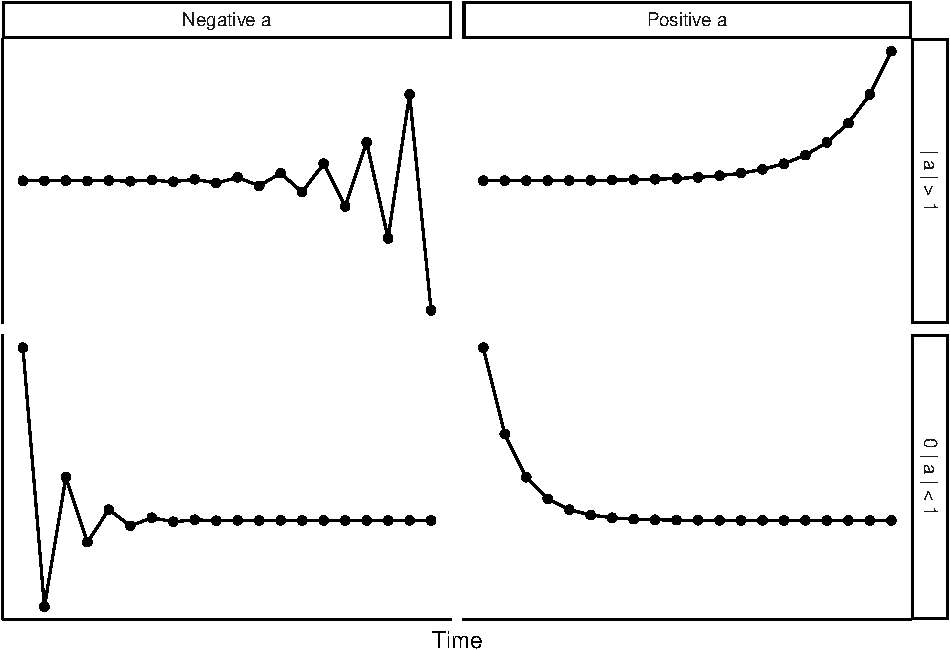
\includegraphics{figs/unnamed-chunk-9-1.pdf}
\caption{\label{fig:unnamed-chunk-9}Trajectories driving toward equilibrium
or explosive behavior based on their autoregressive coefficient. When
the coefficient is greater than one (in absolute value) the trajectory
oscillates explosively or grows exponentially. When the coefficient is
between zero and one (in absolute value) the trajectory converges to
equilibrium.\label{dynamics_plot}}
\end{figure}

\begin{figure}
\centering
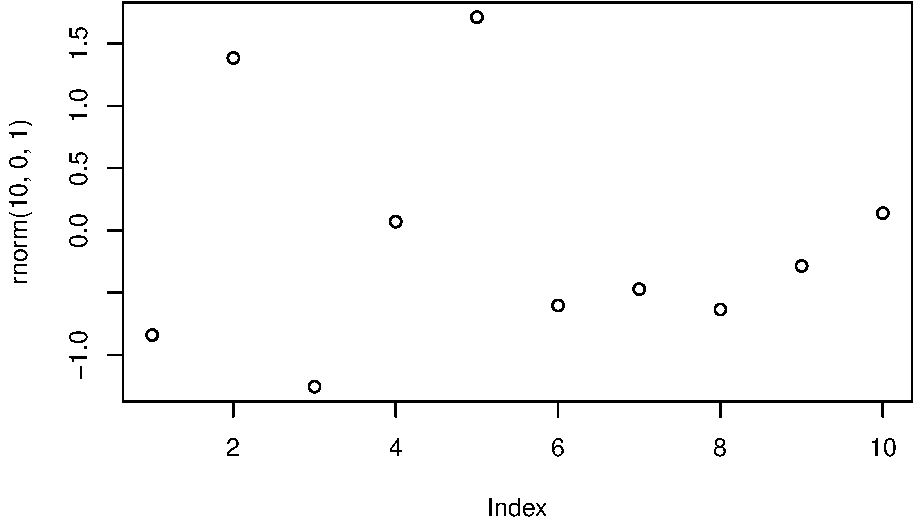
\includegraphics{figs/unnamed-chunk-10-1.pdf}
\caption{\label{fig:unnamed-chunk-10}Two fundamental stochastic processes: a
random walk and white noise.\label{noise}}
\end{figure}

\hypertarget{dynamic-modeling}{%
\subsection{Dynamic Modeling}\label{dynamic-modeling}}

Above, we introduced fundemental concepts for dynamics. Memory,
constraints, initial conditions, equilibrium, reciprocal influence --
these elements constitute the underlying dynamics and are ingredients to
grapple with as researchers consider dynamic phenomenon. Dynamic
mechanisms give rise to observed data, distributions, and statistical
properties for us to witness, and it is those observed data that we
apply models to. In a perfect world researchers could put a magnifying
glass up to their observed data and its statistical properties and
clearly identify the underlying dynamics. Unfortunately we do not live
in that world. Instead, there are a host of challenges that must be
considered when researchers collect longitudinal data and estimate
models to make inferences about dynamics. In this section we describe
stationarity, dynamic panel bias, and ergodicity. Note that throughout
the rest of the paper we replace the layman's term for \(a\)
(self-similarity) with its more common name in the statistical
literature: autoregression, serial correlation, or autocorrelation --
all of these refer to the relationship a state has with itself over
time.

\hypertarget{stationarity}{%
\subsubsection{Stationarity}\label{stationarity}}

States and systems have statistical properties, stationarity is about
the stability of those properties. Rachel's performance across time is
called a time-series -- it is the trajectory of performance for a single
unit (Rachel) over time. That trajectory has properties: it has a mean
and a variance (and autocorrelation or serial correlation). If the mean
is unstable then Rachel's performance either grows or decreases
unconditionally over time. If instead the mean is stable, then Rachel's
performance across time fluctuates but within the constraints of its
memory and bounds on the system. Growth models assume no stationarity in
the data they model, whereas virtually all other models used in the
organizational literature assume that the data they are modeling are
realizations of a stationary process. That is, they assume that the
states and systems they are trying to estimate parameters for have
properties at time \(t\) that are the same as the properties at time
\(t + 1\).

In simple terms, a stationary process has stable properties across time
-- data that demonstrate trend, growth, or random walk behavior are
(almost certainly) non-stationary. Here is the hard part: two
independent time-series will appear related if both are non-stationary
(Granger \& Newbold, 1974; Kuljanin, Braun, \& DeShon, 2011). That is,
if we measure Rachel's performance and it is consistent with a random
walk and we also measure rainfall at Rachel's mother's house across the
state and it demonstrates increasing trend for the day, even though
these two things are completely unrelated we will more than likely find
a relationship between them in a regression-based analysis like those
presented at the start of this paper. There are many other articles that
describe how to test for stationarity (e.g., Braun, Kuljanin, \& DeShon,
2013; Jebb, Tay, Wang, \& Huang, 2015), the point here is to convey how
important this notion is. Our literature is not paying attention to
random walks, we are not checking for memory, or serial correlation, or
stationarity; we should be.

That said, there is a class of models known as cointegration models that
can be used to evaluate relationships in a non-stationary system. These
are more complicated and require a deep understanding of mathematics and
econometric modeling, but interested readers can see Engle and Granger
(1987), Johansen (1991), Phillips (1991), Phillips and Hansen (1990),
and Phillips and Durlauf (1986).

Again, stationarity describes statistical properties that result from
the underlying dynamics. States may or may not have memory, they may or
may not have lag relationships, or reciprocal influence, and may or may
not be constrained by their initial conditions. These aspects are the
underlying dynamics, and the distributions that they give rise to have
properties; stationarity is about those emergent statistical properties.
Any system in equilibrium will be stationary, whereas unstable systems
will be non-stationary. Dynamic processes give rise to distributions and
statistical properties, and those statistical properties create
challenges for models.

\hypertarget{dynamic-panel-bias}{%
\subsubsection{Dynamic Panel Bias}\label{dynamic-panel-bias}}

Another challenge for dynamic modeling is dynamic panel bias, which is
the combined effect of two issues. The first issue has to do with
statistically accounting for memory. Remember that the dynamic equations
above took the form:

\begin{equation}
y_{t} = a y_{t-1} + e_{t}
\end{equation}

\noindent where the only change is that we replaced performance with a
generic \(y\). The equation above has what is called a \enquote{lagged
DV,} where \(y_{t}\) is predicted by the lagged DV: \(y_{t-1}\).
Including lagged DVs helps us \emph{conceptually} represent dynamics
(Keele \& Kelly, 2006), but including a lagged DV in a \emph{model}
applied to data with actual statistical properties causes the errors to
correlate with the predictors and ultimately violate the well-known
independence of errors assumption. This issue applies even when we are
only considering a single unit (like Rachel) across time.

The second issue arises when we are interested in relationships with a
multiple-unit sample across time. Almost all organizational studies are
multiple-unit -- they collect data on more than one participant. If the
people in the sample are not perfectly exchangeable, which means that we
can learn the same thing about performance and fatigue by studying
either Bob or Rachel, we lose no information by restricting our analysis
to one of them, then the parameter estimates are influenced by what is
known as unobserved heterogeneity. Unobserved heterogeneity represents
aggregate, stable individual differences. Rachel's fatigue over time may
look different from Bob's fatigue over time due to unmeasured individual
differences and states. These unacknowledged effects are responsible for
individual differences on fatigue so they need to be incorporated in
statistical models. We acknowledge them by incoporating unobserved
heterogeneity, again it is a term that is meant to represent all of the
unmeasured things that make Rachel's trajectory different from Bob's
trajectory.

In dynamic modeling unobserved heterogeneity must be handled
appropriately: if it is modeled as independent but in fact correlates
with the model predictors then ommitted variables bias is introduced
into the estimates, and if unobserved heterogeneity is ignored then
serial correlation will be introduced into the errors.

Dynamic panel bias is the combined effect of these two biases. Lagged
DVs conceptually convey a dynamic process but they create estimation
problems, and unobserved heterogeneity must be accounted for.
Unfortunately the current workhorse in our literature to examine dynamic
phenomena (the hierarchical linear, random-coefficient, or multi level
model) is not well suited to handle dynamic panel bias. See Xu and
DeShon (current) for a greater discussion of the issue and a recommended
model.

\hypertarget{ergodicity}{%
\subsubsection{Ergodicity}\label{ergodicity}}

In the section above we spoke about unobserved heterogeneity, which can
be thought of as heterogeneity of individual differences or unit
effects. That is, there are unmeasured differences that result in
Rachel's trajectory being different from Bob's. An appropriate next
question is, when is it reasonable to pool Rachel and Bob's data? When
can we be confident that there is homogeneity of dynamics? This is the
notion of ergodicity.

\emph{One more paragraph about it. HELP.}

\hypertarget{discussion---a-dynamic-perspective}{%
\section{Discussion - A Dynamic
Perspective}\label{discussion---a-dynamic-perspective}}

We opened this paper by discussing how researchers are beginning to
approach dynamics. We pointed to two frameworks -- growth and
relationships -- as examples of empirical research doing the hard work
of getting our thinking beyond static, cross-sectional associations.
They were appropriate first steps toward dynamics given our field's
history with random coefficient models and more recent emphasis on
growth curve modeling, but there are many dynamic principles outside the
context of a specific longitudinal model -- we presented them here.
Taking a dynamic perspective means focusing on memory, constraints,
timescales, reciprocal influence, initial conditions, and exploring an
array of satistical properties like serial correlation and stationarity.
Taking a dynamic perspective means being seriously concerned that your
trajectory is not simply a random walk or white noise process.

We close this paper with three short, unique sections to solidify the
principles and what we mean by a dynamic perspective. In the first
section we highlight recent dynamic studies that explore some of the
principles discussed here. Then, we consider what dynamics is not. We
conclude by presenting the linear dynamic systems model as the
fundamental framework for dynamic investigations.

\hypertarget{recent-work}{%
\subsection{Recent Work}\label{recent-work}}

There are several great studies already exploring some of the key
dynamic properties. To get a sense for this literature and to highlight
the principles that they capture, we searched for empirical studies that
were (1) published in the last five years (2) in the \emph{Journal of
Management}, \emph{Journal of Applied Psychology}, or \emph{Academy of
Management Journal} and (3) contained \enquote{dynamic} or
\enquote{dynamics} in the title. We exclude research that is
cross-sectional, ethnographic, or focuses only on growth/covariates of
growth. The articles and the dynamic notions that they emphasize are
listed in Table one.

The studies as a whole explore a number of dynamic principles. First,
every study emphasizes lags -- they evaluate associations, influence,
and patterns from current states to subsequent states, or prior states
to current states. For example, Hardy, Day, and Steele (2018) examine
the relationship between self-efficacy and subsequent exploratory
behavior, the relationship between prior exploratory behavior and
subsequent metacognition, and the relationship between self-efficacy and
subsequent exploratory behavior (among others). Jones et al. (2016)
study the relationship between revealing behaviors among pregnant women
and subsequent physical health symptoms. Many also discuss serial
correlation, autocorrelation, or autoregression. Gabriel and Diefendorff
(2015) assess autocorrelations ranging from T-1 to T-20 seconds, and
their Table one demonstrates how autocorrelation coefficients for
emotion decrease in size over longer lags (i.e., emotions show stronger
self-similarity when they are related to \(t-1\) emotions versus
\(t-20\) emotions). Finally, a number of studies explore reciprocal
patterns over time and a few discuss unobserved heterogeneity indirectly
by using a statistical test to determine if they should employ a fixed
or random effects model (i.e., a Hausman test). These are recent,
exciting dynamic perspectives that our literature is beginning to
expose.

Notice, however, that we also include an \enquote{opportunities} column
in Table one that highlights the principles that could be examined with
the data that currently exist but are not discussed in each article.
Although researchers are thinking about lags and autocorrelation, there
are other principles like initial conditions, equilibrium, timescales,
random walks, stationarity, and endogeneity that have yet to be explored
and are great opportunities to discover even more dynamics. We also
noticed that many of the studies that assess autocorrelation do not have
conceptual discussions about memory or self-similarity or constraints,
but instead assess autocorrelation as a statistical hurdle to overcome
before discussing the lag relationship of interest. It is certainly
appropriate to assess -- especially to avoid inferential errors -- but
finding evidence of memory in a state is useful knowledge on its own and
helps build theoretical understanding.

\begin{center}

---------------

Insert Table 1 Here

---------------

\end{center}

Finally, many of the principles that we highlight as opportunities do
not require grueling extra work. Rather, they can be examined with the
data that already exist to (a) learn more about the system and (b) deter
inferential errors. We hope this paper will ignite more study into the
principles described.

\hypertarget{what-dynamics-is-not}{%
\subsection{What Dynamics Is Not}\label{what-dynamics-is-not}}

During a time when authors were discussing what constitues theory,
Sutton and Staw (1995) produced a useful article describing what theory
is not -- it is a conerstone reading for management, organizational
behavior, human resources, and organizational psychology programs across
the country. A similar approach may be useful here, where addressing
what dynamics is not could help researchers fully grasp its content.

\hypertarget{time-as-a-predictor-is-not-dynamics.}{%
\subsubsection{Time as a predictor is not
dynamics.}\label{time-as-a-predictor-is-not-dynamics.}}

Our field has a number of great papers discussing the idea that time
cannot be causal. Ployhart and colleagues have probably said it best:
\enquote{constructs do not change, evolve, or develop because of time;
rather they do so over time. For example, time does not cause children
to grow into adults. Even though time is highly related to physical
growth, the causes of growth are genetics and environment} (Ployhart \&
Vandenberg, 2010, p. 98). Moreover, our theories do not specify time as
a causal variable but instead specify that changes will happen over time
due to other causes (Pitariu \& Ployhart, 2010).

We agree with these statements but extend them slightly to encompass a
dynamic perspective. Imagine a study that evokes time as a moderator and
then makes a conclusion like, \enquote{early on A happens, whereas later
on B happens.} They do not discuss time as the cause, but they do argue
that they are studying dynamics because state behaviors differ at time 3
compared to time 2. Identifying that time 3 states and relationship
patterns are different from those at time 2 is useful, but it is not
dynamics, it is not characterizing how past behavior constrains new
state patterns or how states from one moment reach others at subsequent
moments. In concrete terms, finding that job satisfaction is high for
newcomers and low for old-timers is not dynamics, neither is recognizing
that it positively relates to performance during week one but negatively
relates to performance after a month on the job. Dynamics is studying
how job satisfaction unfolds through time based on its constraints,
self-similarity, initial conditions, and reciprocal sources of
influence.

\hypertarget{static-relationships-across-time-are-not-dynamics.}{%
\subsubsection{Static relationships across time are not
dynamics.}\label{static-relationships-across-time-are-not-dynamics.}}

Longitudinal data do not automatically make the focus of a study
dynamics. Many studies that collect longitudinal data examine static
relationships across time rather than dynamics, and to see this consider
two simple (mock) examples of studies on burnout and job satisfaction.

The first study collects self reports of burnout and job satisfaction
everyday for three weeks. The researchers regress burnout at time \(t\)
on satisfaction on time \(t\) and report the relationship. Their
analysis, therefore, considers the following relationship:

\begin{equation}
\textrm{Satisfaction}_{t} = a * \textrm{Burnout}_{t} + e_{t}
\end{equation}

\noindent where satisfaction at time 1 is related to burnout at time 1,
satisfaction at time 2 is related to burnout at time 2, and so on.

Now consider a slight change. The researchers instead examine
self-similarity in satisfaction and a lag effect from burnout. That is:

\begin{equation}
\textrm{Satisfaction}_{t} = a * \textrm{Satisfaction}_{t - 1} + b * \textrm{Burnout}_{t - 1} + e_{t}
\end{equation}

\noindent where satisfaction at time 5 is related to its prior self and
burnout at time 4, satisfaction at time 6 is related to satisfaction and
burnout at time 5, and so on.

The only difference between the aforementioned studies is that one
acknowledges memory and lags whereas the other does not, but those
aspects represent and imply fundamentally different things about the
world. The first (equation 15) considers the world as a sequence of
cross-sectional slices, a perspective that Ilgen and Hulin (2000) call
\enquote{multiple snapshots,} where static associations are compiled
across time. It also implies that any state behaviors or relationships
among the states follow a seemingly odd sequence: relationships happen
at one moment and then are wiped out and replaced by completely new
behavior and relationship patterns at the next. Finally, it represents a
world where burnout instantaneously causes satisfaction. Virtually all
studies that use a time-varying covariates model adopt this perspective.

The second, dynamic perspective (equation 16) represents a much
different structure. Satisfaction is constrained by where it was in the
past and therefore it cannot bounce to extreme levels without first
moving from its prior state. Moreover, the effect from burnout takes
time to occur and aligns with intuitive and theoretical notions of
causality. Finally, the patterns between satisfaction and burnout will
ultimately drive toward equilibrium. A study of relationships over time
is useful, but it is not dynamics.

\hypertarget{dynamics-is-not-synonymous-with-growth.}{%
\subsubsection{Dynamics is not synonymous with
growth.}\label{dynamics-is-not-synonymous-with-growth.}}

A dynamic phenomenon does not have to grow or exhibit
increasing/decreasing trend. The underlying dynamics may or may not
produce trend, but growth is not a fundamental concept in dynamics.
Similarly, observing growth or correlates of growth in an empirical
study is not dynamics. It is useful and we hope researchers continue to
explore growth patterns in their content areas, but a study that
\enquote{unpacks dynamics} is much different from a study that estimates
trend and predictors of trend.

\hypertarget{conclusion---the-linear-dynamic-systems-model}{%
\subsection{Conclusion - The Linear Dynamic Systems
Model}\label{conclusion---the-linear-dynamic-systems-model}}

Much of the historical research in our field emphasized bivariate,
cross-sectional relationships that are embodied in the general linear
model. As we incorporate dynamics, there are a number of additional
principles to consider and we discussed many of them in this paper. The
principles of dynamics are all represented in a different fundamental
model: the linear dynamic systems model. Just as the general linear
model subsumes historical research focused on static relationships, the
linear dynamic systems model will embody our upcoming dynamic
investigations. In its simplest form, the linear dynamic sytems model
is:

\begin{equation}
\textbf{x}_t = \textbf{A} \textbf{x}_{t-1} + \textbf{b}
\end{equation}

\noindent where \textbf{x}\(_t\) is a vector of states at time \(t\).
The vector is just like the state vector we presented in the concepts
section (depletion, fatigue, burnout), but here we use a generic term to
capture any state or set of states of interest. The equation also
captures the states at the prior time point, \textbf{x}\(_{t-1}\), and
those states are multiplied by \textbf{A}, a matrix of transition
weights. The transition weights capture memory, constraints, lags, and
reciprocal influence within the system -- the diagonal elements
represent self-similarity and the off-diagonal elements are cross-state
influence. \textbf{b} is a vector of constant values (time-invariant)
that are commonly referred to as forcing terms. Although they do not
receive a term in the equation, initial conditions are also inherent to
the linear dynamic systems model because specifying or identifying a
trajectory requires starting values. The principles described in this
paper are embodied in the linear dynamic systems model and it will serve
as the underlying model as we enter the exciting domain of dynamics.

\begin{longtable}[t]{>{\raggedright\arraybackslash}p{10em}>{\raggedright\arraybackslash}p{11em}>{\raggedright\arraybackslash}p{20em}}
\caption{\label{tab:unnamed-chunk-11}\label{highlight}Recent studies exploring dynamic notions.}\\
\toprule
Article & Dynamic Notions & Opportunities\\
\midrule
\endfirsthead
\caption[]{\label{tab:unnamed-chunk-11}Recent studies exploring dynamic notions. \textit{(continued)}}\\
\toprule
Article & Dynamic Notions & Opportunities\\
\midrule
\endhead
\
\endfoot
\bottomrule
\endlastfoot
\begingroup\fontsize{12}{14}\selectfont Berrone, Gelabert, Massa-Saluzzo, and Rousseau, 2016\endgroup & \begingroup\fontsize{12}{14}\selectfont Unobserved heterogeneity\newline Lags\endgroup & \begingroup\fontsize{12}{14}\selectfont Initial conditions\newline Memory\newline Timescales\newline Boundary conditions\newline Reciprocal relationships\newline Equilibrium\newline Random walks and white noise\newline Stationarity\newline Endogeneity\endgroup\\
\hline
\begingroup\fontsize{12}{14}\selectfont Call, Nyberg, Ployhart, and Weekley, 2015\endgroup & \begingroup\fontsize{12}{14}\selectfont Unobserved heterogeneity\newline Lags\newline Serial correlation\newline Timescales\endgroup & \begingroup\fontsize{12}{14}\selectfont Initial conditions\newline Boundary conditions\newline Reciprocal relationships\newline Equilibrium\newline Random walks and white noise\newline Stationarity\newline Endogeneity\endgroup\\
\hline
\begingroup\fontsize{12}{14}\selectfont Drescher, Korsgaard, Welpe, Picot, and Wigand, 2014\endgroup & \begingroup\fontsize{12}{14}\selectfont Lags\newline Autocorrelation\endgroup & \begingroup\fontsize{12}{14}\selectfont Initial conditions\newline Timescales\newline Boundary conditions\newline Reciprocal relationships\newline Equilibrium\newline Random walks and white noise\newline Unobserved heterogeneity\newline Stationarity\newline Endogeneity\endgroup\\
\hline
\begingroup\fontsize{12}{14}\selectfont Gabriel and Diefendorff, 2015\endgroup & \begingroup\fontsize{12}{14}\selectfont Lags\newline Autocorrelation\newline Reciprocal relationships\newline Timescales\endgroup & \begingroup\fontsize{12}{14}\selectfont Initial conditions\newline Boundary conditions\newline Equilibrium\newline Random walks and white noise\newline Unobserved heterogeneity\newline Stationarity\newline Endogeneity\endgroup\\
\hline
\begingroup\fontsize{12}{14}\selectfont Hardy, Day, and Steele, 2018\endgroup & \begingroup\fontsize{12}{14}\selectfont Lags\newline Reciprocal relationships\endgroup & \begingroup\fontsize{12}{14}\selectfont Initial conditions\newline Memory\newline Timescales\newline Boundary conditions\newline Equilibrium\newline Random walks and white noise\newline Unobserved heterogeneity\newline Stationarity\newline Endogeneity\endgroup\\
\hline
\addlinespace
\begingroup\fontsize{12}{14}\selectfont Jones, King, Gilrane, McCausland, Cortina, and Grimm, 2013\endgroup & \begingroup\fontsize{12}{14}\selectfont Lags\newline Autocorrelation\newline Reciprocal relationships\endgroup & \begingroup\fontsize{12}{14}\selectfont Initial conditions\newline Timescales\newline Boundary conditions\newline Equilibrium\newline Random walks and white noise\newline Unobserved heterogeneity\newline Stationarity\newline Endogeneity\endgroup\\
\hline
\begingroup\fontsize{12}{14}\selectfont Taylor, Bedeian, Cole, and Zhang, 2014\endgroup & \begingroup\fontsize{12}{14}\selectfont Lags\newline Autocorrelation\newline Reciprocal relationships\endgroup & \begingroup\fontsize{12}{14}\selectfont Initial conditions\newline Timescales\newline Boundary conditions\newline Equilibrium\newline Random walks and white noise\newline Unobserved heterogeneity\newline Stationarity\newline Endogeneity\endgroup\\
\hline
\begingroup\fontsize{12}{14}\selectfont Tepper, Dimotakis, Lambert, Koopman, Matta, Park, and Goo, 2018\endgroup & \begingroup\fontsize{12}{14}\selectfont Lags\newline Autoregression\endgroup & \begingroup\fontsize{12}{14}\selectfont Initial conditions\newline Timescales\newline Boundary conditions\newline Equilibrium\newline Reciprocal relationships\newline Random walks and white noise\newline Unobserved heterogeneity\newline Stationarity\newline Endogeneity\endgroup\\*
\end{longtable}

\newpage

\hypertarget{references}{%
\section{References}\label{references}}

\setlength{\parindent}{-0.5in}
\setlength{\leftskip}{0.5in}

\hypertarget{refs}{}
\leavevmode\hypertarget{ref-beck2013state}{}%
Beck, J. W., \& Schmidt, A. M. (2013). State-level goal orientations as
mediators of the relationship between time pressure and performance: A
longitudinal study. \emph{Journal of Applied Psychology}, \emph{98}(2),
354.

\leavevmode\hypertarget{ref-boulding1955defense}{}%
Boulding, K. E. (1955). In defense of statics. \emph{The Quarterly
Journal of Economics}, \emph{69}(4), 485--502.

\leavevmode\hypertarget{ref-braun_spurious_2013}{}%
Braun, M. T., Kuljanin, G., \& DeShon, R. P. (2013). Spurious Results in
the Analysis of Longitudinal Data in Organizational Research.
\emph{Organizational Research Methods}, \emph{16}(2), 302--330.
doi:\href{https://doi.org/10.1177/1094428112469668}{10.1177/1094428112469668}

\leavevmode\hypertarget{ref-cronin2009don}{}%
Cronin, M. A., Gonzalez, C., \& Sterman, J. D. (2009). Why don't
well-educated adults understand accumulation? A challenge to
researchers, educators, and citizens. \emph{Organizational Behavior and
Human Decision Processes}, \emph{108}(1), 116--130.

\leavevmode\hypertarget{ref-dalal2015personality}{}%
Dalal, R. S., Meyer, R. D., Bradshaw, R. P., Green, J. P., Kelly, E. D.,
\& Zhu, M. (2015). Personality strength and situational influences on
behavior: A conceptual review and research agenda. \emph{Journal of
Management}, \emph{41}(1), 261--287.

\leavevmode\hypertarget{ref-dragoni2005understanding}{}%
Dragoni, L. (2005). Understanding the emergence of state goal
orientation in organizational work groups: The role of leadership and
multilevel climate perceptions. \emph{Journal of Applied Psychology},
\emph{90}(6), 1084.

\leavevmode\hypertarget{ref-dunford_is_2012}{}%
Dunford, B. B., Shipp, A. J., Boss, R. W., Angermeier, I., \& Boss, A.
D. (2012). Is burnout static or dynamic? A career transition perspective
of employee burnout trajectories. \emph{Journal of Applied Psychology},
\emph{97}(3), 637--650.
doi:\href{https://doi.org/http://dx.doi.org.proxy2.cl.msu.edu/10.1037/a0027060}{http://dx.doi.org.proxy2.cl.msu.edu/10.1037/a0027060}

\leavevmode\hypertarget{ref-engle_co-integration_1987}{}%
Engle, R. F., \& Granger, C. W. (1987). Co-integration and error
correction: Representation, estimation, and testing. \emph{Econometrica:
Journal of the Econometric Society}, 251--276.

\leavevmode\hypertarget{ref-flytzanis1976linear}{}%
Flytzanis, E. (1976). Linear dynamical systems. \emph{Proceedings of the
American Mathematical Society}, \emph{55}(2), 367--370.

\leavevmode\hypertarget{ref-gabriel_emotional_2015}{}%
Gabriel, A. S., \& Diefendorff, J. M. (2015). Emotional labor dynamics:
A momentary approach. \emph{Academy of Management Journal},
\emph{58}(6), 1804--1825.

\leavevmode\hypertarget{ref-gabriel_helping_2018}{}%
Gabriel, A. S., Koopman, J., Rosen, C. C., \& Johnson, R. E. (2018).
Helping others or helping oneself? An episodic examination of the
behavioral consequences of helping at work. \emph{Personnel Psychology},
\emph{71}(1), 85--107.

\leavevmode\hypertarget{ref-granger_spurious_1974}{}%
Granger, C. W., \& Newbold, P. (1974). Spurious regressions in
econometrics. \emph{Journal of Econometrics}, \emph{2}(2), 111--120.

\leavevmode\hypertarget{ref-hamaker2007integrated}{}%
Hamaker, E. L., Nesselroade, J. R., \& Molenaar, P. C. (2007). The
integrated trait--state model. \emph{Journal of Research in
Personality}, \emph{41}(2), 295--315.

\leavevmode\hypertarget{ref-hardy_interrelationships_2018}{}%
Hardy, J. H., Day, E. A., \& Steele, L. M. (2018). Interrelationships
Among Self-Regulated Learning Processes: Toward a Dynamic Process-Based
Model of Self-Regulated Learning. \emph{Journal of Management},
0149206318780440.
doi:\href{https://doi.org/10.1177/0149206318780440}{10.1177/0149206318780440}

\leavevmode\hypertarget{ref-hulsheger_dawn_2016}{}%
Hülsheger, U. R. (2016). From dawn till dusk: Shedding light on the
recovery process by investigating daily change patterns in fatigue.
\emph{Journal of Applied Psychology}, \emph{101}(6), 905--914.
doi:\href{https://doi.org/http://dx.doi.org.proxy2.cl.msu.edu/10.1037/apl0000104}{http://dx.doi.org.proxy2.cl.msu.edu/10.1037/apl0000104}

\leavevmode\hypertarget{ref-ilgen_computational_2000}{}%
Ilgen, D. R., \& Hulin, C. L. (2000). \emph{Computational modeling of
behavior in organizations: The third scientific discipline.} American
Psychological Association.

\leavevmode\hypertarget{ref-james1982causal}{}%
James, L., Mulaik, S., \& Brett, J. M. (1982). \emph{Causal analysis:
Assumptions, models, and data}. Newbury Park, CA: Sage publications.

\leavevmode\hypertarget{ref-jebb_time_2015}{}%
Jebb, A. T., Tay, L., Wang, W., \& Huang, Q. (2015). Time series
analysis for psychological research: Examining and forecasting change.
\emph{Frontiers in Psychology}, \emph{6}, 727.

\leavevmode\hypertarget{ref-johansen_estimation_1991}{}%
Johansen, S. (1991). Estimation and hypothesis testing of cointegration
vectors in Gaussian vector autoregressive models. \emph{Econometrica:
Journal of the Econometric Society}, 1551--1580.

\leavevmode\hypertarget{ref-johnson_good_2014}{}%
Johnson, R. E., Lanaj, K., \& Barnes, C. M. (2014). The good and bad of
being fair: Effects of procedural and interpersonal justice behaviors on
regulatory resources. \emph{Journal of Applied Psychology},
\emph{99}(4), 635.

\leavevmode\hypertarget{ref-jones_baby_2016}{}%
Jones, K. P., King, E. B., Gilrane, V. L., McCausland, T. C., Cortina,
J. M., \& Grimm, K. J. (2016). The baby bump: Managing a dynamic stigma
over time. \emph{Journal of Management}, \emph{42}(6), 1530--1556.

\leavevmode\hypertarget{ref-keele_dynamic_2006}{}%
Keele, L., \& Kelly, N. J. (2006). Dynamic models for dynamic theories:
The ins and outs of lagged dependent variables. \emph{Political
Analysis}, \emph{14}(2), 186--205.

\leavevmode\hypertarget{ref-kenny1979correlation}{}%
Kenny, D. A. (1979). \emph{Correlation and causality}. \emph{New York:
Wiley}.

\leavevmode\hypertarget{ref-koopman_integrating_2016}{}%
Koopman, J., Lanaj, K., \& Scott, B. A. (2016). Integrating the Bright
and Dark Sides of OCB: A Daily Investigation of the Benefits and Costs
of Helping Others. \emph{Academy of Management Journal}, \emph{59}(2),
414--435.
doi:\href{https://doi.org/10.5465/amj.2014.0262}{10.5465/amj.2014.0262}

\leavevmode\hypertarget{ref-kuljanin_cautionary_2011}{}%
Kuljanin, G., Braun, M. T., \& DeShon, R. P. (2011). A cautionary note
on modeling growth trends in longitudinal data. \emph{Psychological
Methods}, \emph{16}(3), 249--264.
doi:\href{https://doi.org/http://dx.doi.org.proxy2.cl.msu.edu/10.1037/a0023348}{http://dx.doi.org.proxy2.cl.msu.edu/10.1037/a0023348}

\leavevmode\hypertarget{ref-liebovitch2010dynamics}{}%
Liebovitch, L. S., Vallacher, R. R., \& Michaels, J. (2010). Dynamics of
cooperation--competition interaction models. \emph{Peace and Conflict},
\emph{16}(2), 175--188.

\leavevmode\hypertarget{ref-mathieu2006clarifying}{}%
Mathieu, J. E., \& Taylor, S. R. (2006). Clarifying conditions and
decision points for mediational type inferences in organizational
behavior. \emph{Journal of Organizational Behavior: The International
Journal of Industrial, Occupational and Organizational Psychology and
Behavior}, \emph{27}(8), 1031--1056.

\leavevmode\hypertarget{ref-miner2010state}{}%
Miner, A. G., \& Glomb, T. M. (2010). State mood, task performance, and
behavior at work: A within-persons approach. \emph{Organizational
Behavior and Human Decision Processes}, \emph{112}(1), 43--57.

\leavevmode\hypertarget{ref-monge_theoretical_1990}{}%
Monge, P. R. (1990). Theoretical and analytical issues in studying
organizational processes. \emph{Organization Science}, \emph{1}(4),
406--430.

\leavevmode\hypertarget{ref-phillips_optimal_1991}{}%
Phillips, P. C. (1991). Optimal inference in cointegrated systems.
\emph{Econometrica: Journal of the Econometric Society}, 283--306.

\leavevmode\hypertarget{ref-phillips_multiple_1986}{}%
Phillips, P. C., \& Durlauf, S. N. (1986). Multiple time series
regression with integrated processes. \emph{The Review of Economic
Studies}, \emph{53}(4), 473--495.

\leavevmode\hypertarget{ref-phillips_statistical_1990}{}%
Phillips, P. C., \& Hansen, B. E. (1990). Statistical inference in
instrumental variables regression with I (1) processes. \emph{The Review
of Economic Studies}, \emph{57}(1), 99--125.

\leavevmode\hypertarget{ref-pitariu_explaining_2010}{}%
Pitariu, A. H., \& Ployhart, R. E. (2010). Explaining change: Theorizing
and testing dynamic mediated longitudinal relationships. \emph{Journal
of Management}, \emph{36}(2), 405--429.

\leavevmode\hypertarget{ref-ployhart_longitudinal_2010}{}%
Ployhart, R. E., \& Vandenberg, R. J. (2010). Longitudinal research: The
theory, design, and analysis of change. \emph{Journal of Management},
\emph{36}(1), 94--120.

\leavevmode\hypertarget{ref-rosen_who_2016}{}%
Rosen, C. C., Koopman, J., Gabriel, A. S., \& Johnson, R. E. (2016). Who
strikes back? A daily investigation of when and why incivility begets
incivility. \emph{Journal of Applied Psychology}, \emph{101}(11), 1620.

\leavevmode\hypertarget{ref-simon1991architecture}{}%
Simon, H. A. (1991). The architecture of complexity. In \emph{Facets of
systems science} (pp. 457--476). Springer.

\leavevmode\hypertarget{ref-sutton1995theory}{}%
Sutton, R. I., \& Staw, B. M. (1995). What theory is not.
\emph{Administrative Science Quarterly}, 371--384.

\leavevmode\hypertarget{ref-vancouver_translating_2018}{}%
Vancouver, J. B., Wang, M., \& Li, X. (2018). Translating Informal
Theories Into Formal Theories: The Case of the Dynamic Computational
Model of the Integrated Model of Work Motivation. \emph{Organizational
Research Methods}, 109442811878030.
doi:\href{https://doi.org/10.1177/1094428118780308}{10.1177/1094428118780308}


\end{document}
